\chapter{Misturas Heterogêneas: Equilíbrio de Fases}
\label{chap:heterogeneousMixtures}

    Até esta parte do nosso estudo, adquirimos a capacidade de resolver
    qualquer tipo de problema que possa ser modelado como misturas homogêneas,
    seja considerando-as como solução ideal, seja tratando-as como
    pseudo-substâncias puras e lançando mão de um modelo pseudo-crítico
    apropriado. Resta-nos a questão: \emph{o que fazer quando a mistura for
    heterogênea?} Mesmo se não tenhamos a resposta ao problema mais geral, pelo
    menos um caso de mistura nestas condições vale a pena abordar: a mistura em
    equilíbrio de fases.

    Seja então o sistema fechado binário bifásico à temperatura
    \gls{temperature} e pressão \gls{pressure} uniformes, contendo
    \propcomp{numberMoles}{A} moles de A e \propcomp{numberMoles}{B} moles de
    B, sendo que cada fase (1) e (2) contém ambas as substâncias A e B.
    \emph{Determine as condições pelas quais há equilíbrio de fases.}

    A fração molar de cada componente em cada fase será dada por:
    %
    \begin{equation} \label{eq:9.1}
        \phase{\propcomp{moleFraction}{A}}{1}
        =
        \frac{
            \phase{\propcomp{numberMoles}{A}}{1}
        }{
            \phase{\propcomp{numberMoles}{A}}{1}
            +
            \phase{\propcomp{numberMoles}{B}}{1}
        }\,,
    \end{equation}
    %
    \begin{equation} \label{eq:9.2}
        \phase{\propcomp{moleFraction}{B}}{1}
        =
        \frac{
            \phase{\propcomp{numberMoles}{B}}{1}
        }{
            \phase{\propcomp{numberMoles}{A}}{1}
            +
            \phase{\propcomp{numberMoles}{B}}{1}
        }\,,
    \end{equation}
    %
    \begin{equation} \label{eq:9.3}
        \phase{\propcomp{moleFraction}{A}}{2}
        =
        \frac{
            \phase{\propcomp{numberMoles}{A}}{2}
        }{
            \phase{\propcomp{numberMoles}{A}}{2}
            +
            \phase{\propcomp{numberMoles}{B}}{2}
        }\,,
    \end{equation}
    %
    e
    %
    \begin{equation} \label{eq:9.4}
        \phase{\propcomp{moleFraction}{B}}{2}
        =
        \frac{
            \phase{\propcomp{numberMoles}{B}}{2}
        }{
            \phase{\propcomp{numberMoles}{A}}{2}
            +
            \phase{\propcomp{numberMoles}{B}}{2}
        }\,.
    \end{equation}

    Claramente,
    %
    \begin{equation} \label{eq:9.5}
        \phase{\propcomp{moleFraction}{A}}{1}
        +
        \phase{\propcomp{moleFraction}{B}}{1}
        =
        1\,,
        \,\,\,\,
        \text{e}
        \,\,\,\,
        \phase{\propcomp{moleFraction}{A}}{2}
        +
        \phase{\propcomp{moleFraction}{B}}{2}
        =
        1\,,
    \end{equation}
    %
    mas veremos que a relação entre \phase{\propcomp{moleFraction}{A}}{1} e
    \phase{\propcomp{moleFraction}{A}}{2} ou então entre
    \phase{\propcomp{moleFraction}{B}}{1} e
    \phase{\propcomp{moleFraction}{B}}{2} não é nada trivial, muito ao
    contrário, pertence à essência  do que vamos estudar agora.

    Quando se fixa a temperatura e a pressão de um sistema, a propriedade
    termodinâmica natural para se analisar o seu comportamento é a função (ou
    energia livre) de Gibbs. Pode-se mostrar que com \gls{temperature} e
    \gls{pressure} constantes, o sistema irá se aproximar do equilíbrio através
    da minimização da função de Gibbs total G da mistura. Como cada fase é uma
    mistura homogênea, podemos escrever:
    %
    \begin{equation} \label{eq:9.6}
        \phase{\gls{GibbsFreeEnergy}}{1}
        =
        \phase{\gls{GibbsFreeEnergy}}{1}
        \functionOf{
            \gls{temperature},\gls{pressure},
            \phase{\propcomp{numberMoles}{A}}{1},
            \phase{\propcomp{numberMoles}{B}}{1}
        }\,,
        \,\,\,\,
        %
        \text{e}
        %
        \phase{\gls{GibbsFreeEnergy}}{2}
        =
        \phase{\gls{GibbsFreeEnergy}}{2}
        \functionOf{
            \gls{temperature},\gls{pressure},
            \phase{\propcomp{numberMoles}{A}}{2},
            \phase{\propcomp{numberMoles}{B}}{2}
        }\,,
    \end{equation}
    %
    e pela regra da cadeia,
    %
    \begin{equation} \label{eq:9.7}
        \diff{\phase{\gls{GibbsFreeEnergy}}{1}}
        =
        \ddxconsty{
            \phase{\gls{GibbsFreeEnergy}}{1}
        }{
            \gls{temperature}
        }{
            \gls{pressure},
            \phase{\propcomp{numberMoles}{A}}{1},
            \phase{\propcomp{numberMoles}{B}}{1}
        }
        \diff{\gls{temperature}}
        +
        \ddxconsty{
            \phase{\gls{GibbsFreeEnergy}}{1}
        }{
            \gls{pressure}
        }{
            \gls{temperature},
            \phase{\propcomp{numberMoles}{A}}{1},
            \phase{\propcomp{numberMoles}{B}}{1}
        }
        \diff{\gls{pressure}}\\
        +
        \ddxconsty{
            \phase{\gls{GibbsFreeEnergy}}{1}
        }{
            \phase{\propcomp{numberMoles}{A}}{1}
        }{
            \gls{temperature},
            \gls{pressure},
            \phase{\propcomp{numberMoles}{B}}{1}
        }
        \diff{\phase{\propcomp{numberMoles}{A}}{1}}
        +
        \ddxconsty{
            \phase{\gls{GibbsFreeEnergy}}{1}
        }{
            \phase{\propcomp{numberMoles}{B}}{1}
        }{
            \gls{temperature},
            \gls{pressure},
            \phase{\propcomp{numberMoles}{A}}{1}
        }
        \diff{\phase{\propcomp{numberMoles}{B}}{1}}\,,
    \end{equation}
    %
    \begin{equation} \label{eq:9.8}
        \diff{\phase{\gls{GibbsFreeEnergy}}{2}}
        =
        \ddxconsty{
            \phase{\gls{GibbsFreeEnergy}}{2}
        }{
            \gls{temperature}
        }{
            \gls{pressure},
            \phase{\propcomp{numberMoles}{A}}{2},
            \phase{\propcomp{numberMoles}{B}}{2}
        }
        \diff{\gls{temperature}}
        +
        \ddxconsty{
            \phase{\gls{GibbsFreeEnergy}}{2}
        }{
            \gls{pressure}
        }{
            \gls{temperature},
            \phase{\propcomp{numberMoles}{A}}{2},
            \phase{\propcomp{numberMoles}{B}}{2}
        }
        \diff{\gls{pressure}}\\
        +
        \ddxconsty{
            \phase{\gls{GibbsFreeEnergy}}{2}
        }{
            \phase{\propcomp{numberMoles}{A}}{2}
        }{
            \gls{temperature},
            \gls{pressure},
            \phase{\propcomp{numberMoles}{B}}{2}
        }
        \diff{\phase{\propcomp{numberMoles}{A}}{2}}
        +
        \ddxconsty{
            \phase{\gls{GibbsFreeEnergy}}{2}
        }{
            \phase{\propcomp{numberMoles}{B}}{2}
        }{
            \gls{temperature},
            \gls{pressure},
            \phase{\propcomp{numberMoles}{A}}{2}
        }
        \diff{\phase{\propcomp{numberMoles}{B}}{2}}\,.
    \end{equation}

    Observe que, conforme aprendemos, os dois últimos termos de cada equação
    definem a função de Gibbs parcial molar de cada componente em cada fase (1)
    e (2). Além disso, vamos manter a temperatura e a pressão constantes para
    analisar o efeito sobre a função de Gibbs total do sistema provocado pela
    variação das concentrações dos componentes nas fases. Podemos, então,
    escrever
    %
    \begin{equation} \label{eq:9.9}
        \begin{aligned}
            \diff{\gls{GibbsFreeEnergy}}_{\gls{temperature},\gls{pressure}}
            =
            \diff{
                \phase{\gls{GibbsFreeEnergy}}{1}
            }_{\gls{temperature},\gls{pressure}}
            +
            \diff{
                \phase{\gls{GibbsFreeEnergy}}{2}
            }_{\gls{temperature},\gls{pressure}}
            =&
            \phase{\partmolalprop{GibbsFreeEnergy}{A}}{1}
            \functionOf{
                \gls{temperature},
                \gls{pressure},
                \phase{\propcomp{moleFraction}{A}}{1}
            }
            \diff{
                \phase{\propcomp{numberMoles}{A}}{1}
            }
            +
            \phase{\partmolalprop{GibbsFreeEnergy}{B}}{1}
            \functionOf{
                \gls{temperature},
                \gls{pressure},
                \phase{\propcomp{moleFraction}{A}}{1}
            }
            \diff{
                \phase{\propcomp{numberMoles}{B}}{1}
            }
            +\\
            &\phase{\partmolalprop{GibbsFreeEnergy}{A}}{2}
            \functionOf{
                \gls{temperature},
                \gls{pressure},
                \phase{\propcomp{moleFraction}{A}}{2}
            }
            \diff{
                \phase{\propcomp{numberMoles}{A}}{2}
            }
            +
            \phase{\partmolalprop{GibbsFreeEnergy}{B}}{2}
            \functionOf{
                \gls{temperature},
                \gls{pressure},
                \phase{\propcomp{moleFraction}{A}}{2}
            }
            \diff{
                \phase{\propcomp{numberMoles}{B}}{2}
            }\,.
        \end{aligned}
    \end{equation}

    A propósito, o coeficiente de \diff{\propcomp{numberMoles}{i}} para cada
    componente $i$ é o potencial de transferência de massa do componente $i$ na
    mistura, denominado potencial químico (ou eletroquímico)
    \propcomp{chemicalPotential}{i} do componente $i$ na mistura a
    \gls{temperature} e \gls{pressure}. Se o equilíbrio térmico é a igualdade
    de temperaturas e o equilíbrio mecânico é a igualdade de pressões, podemos
    supor que o equilíbrio químico será dado pela igualdade de potenciais
    químicos do componente. De uma discussão anterior, você pode verificar que
    o potencial químico coincide com a função de Gibbs parcial molar e, de
    fato, ambos podem ser usados intercambiavelmente. (Será que o potencial
    químico pode ser igual a entalpia parcial molar, por exemplo?)

    Bem, o que temos aqui? Qualquer decréscimo de A em (1)
    ($\diff{\phase{\propcomp{numberMoles}{A}}{1}} < 0$) deve ser acompanhado de
    um aumento de A idêntico em (2)
    ($\diff{\phase{\propcomp{numberMoles}{A}}{2}} =
    -\diff{\phase{\propcomp{numberMoles}{A}}{1}}$) e analogamente para B.
    Portanto,
    %
    \begin{equation} \label{eq:9.10}
        \diff{
            \gls{GibbsFreeEnergy}
        }_{\gls{temperature},\gls{pressure}}
        =
        \left[
            \phase{\partmolalprop{GibbsFreeEnergy}{A}}{1}
            -
            \phase{\partmolalprop{GibbsFreeEnergy}{A}}{2}
        \right]
        \diff{
            \phase{\propcomp{numberMoles}{A}}{1}
        }
        +
        \left[
            \phase{\partmolalprop{GibbsFreeEnergy}{B}}{1}
            -
            \phase{\partmolalprop{GibbsFreeEnergy}{B}}{2}
        \right]
        \diff{
            \phase{\propcomp{numberMoles}{B}}{1}
        }\,,
    \end{equation}
    %
    de modo que \diff{\phase{\propcomp{numberMoles}{A}}{1}} e
    \diff{\phase{\propcomp{numberMoles}{B}}{1}} são verdadeiramente
    independentes.  No equilíbrio, desde que \gls{temperature}, \gls{pressure}
    sejam constantes, a composição das fases não mais se altera. Para obter-se
    o equilíbrio, a minimização da função de Gibbs do sistema exige que
    $\diff{\gls{GibbsFreeEnergy}}_{\gls{temperature},\gls{pressure}} = 0$ e,
    portanto, concluímos que
    %
    \begin{equation} \label{eq:9.11}
        \phase{\partmolalprop{GibbsFreeEnergy}{A}}{1}
        \functionOf{
            \gls{temperature},
            \gls{pressure},
            \phase{\propcomp{moleFraction}{A}}{1}
        }
        =
        \phase{\partmolalprop{GibbsFreeEnergy}{A}}{2}
        \functionOf{
            \gls{temperature},
            \gls{pressure},
            \phase{\propcomp{moleFraction}{A}}{2}
        }\,,
    \end{equation}
    %
    \begin{equation} \label{eq:9.12}
        \phase{\partmolalprop{GibbsFreeEnergy}{B}}{1}
        \functionOf{
            \gls{temperature},
            \gls{pressure},
            \phase{\propcomp{moleFraction}{A}}{1}
        }
        =
        \phase{\partmolalprop{GibbsFreeEnergy}{B}}{2}
        \functionOf{
            \gls{temperature},
            \gls{pressure},
            \phase{\propcomp{moleFraction}{A}}{2}
        }\,.
    \end{equation}

    A forma funcional ressalta que temos quatro variáveis independentes
    $\gls{temperature}, \gls{pressure}, \phase{\propcomp{moleFraction}{A}}{1},
    \phase{\propcomp{moleFraction}{A}}{2}$ porém, somente duas equações! Isso
    quer dizer que, para que possamos resolver este sistema de equações, temos
    que fornecer o valor de quaisquer duas destas variáveis. Vamos supor que
    fornecemos \gls{temperature} e \gls{pressure}. Então, todas as demais
    variáveis estarão determinadas pela solução do sistema de equações dado
    pelas \cref{eq:9.11,eq:9.12}.

    De um modo geral, seja uma mistura a \gls{temperature} e \gls{pressure} com
    \gls{numberPhases} fases e \gls{numberSpecies} componentes, cada um destes
    fazendo parte da composição da mistura homogênea em cada uma das fases. A
    fração molar de cada componente $i$ em cada fase $j$ será dada por:
    %
    \begin{equation} \label{eq:9.13}
        \phase{\propcomp{moleFraction}{i}}{j}
        =
        \frac{
            \phase{\propcomp{numberMoles}{i}}{j}
        }{
            \sum\limits_{i = 1}{\gls{numberSpecies}}{
                \phase{\propcomp{numberMoles}{i}}{j}
            }
        }\,,
    \end{equation}
    %
    para cada componente $i$ de cada fase $j$.

    As variáveis independentes para esta mistura passam a ser
    %
    \begin{equation*}
        \gls{temperature},
        \gls{pressure},
        \phase{\propcomp{moleFraction}{1}}{1},
        \phase{\propcomp{moleFraction}{2}}{1},
        \hdots,
        \phase{\propcomp{moleFraction}{\gls{numberSpecies} - 1}}{1},
        \phase{\propcomp{moleFraction}{1}}{2},
        \phase{\propcomp{moleFraction}{2}}{2},
        \hdots,
        \phase{\propcomp{moleFraction}{\gls{numberSpecies} - 1}}{2},
        \hdots,
        \phase{\propcomp{moleFraction}{1}}{\gls{numberPhases}},
        \phase{\propcomp{moleFraction}{2}}{\gls{numberPhases}},
        \hdots,
        \phase{
            \propcomp{moleFraction}{\gls{numberSpecies} - 1}
        }{\gls{numberPhases}}\,,
    \end{equation*}
    %
    cujo total é de $\gls{numberPhases}(\gls{numberSpecies} - 1) + 2$
    incógnitas (por quê?). O sistema de  equações, por sua vez, será dado pelas
    igualdades dos potenciais químicos de cada componente em cada fase:
    %
    \begin{equation} \label{eq:9.14}
        \begin{aligned}
            &\phase{\propcomp{chemicalPotential}{1}}{1}
            \functionOf{
                \gls{temperature},
                \gls{pressure},
                \phase{\propcomp{moleFraction}{1}}{1},
                \hdots,
                \phase{
                    \propcomp{moleFraction}{\gls{numberSpecies} - 1}
                }{1}
            }
            =
            \phase{\propcomp{chemicalPotential}{1}}{2}
            \functionOf{
                \gls{temperature},
                \gls{pressure},
                \phase{\propcomp{moleFraction}{1}}{2},
                \hdots,
                \phase{
                    \propcomp{moleFraction}{\gls{numberSpecies} - 1}
                }{2}
            }
            =
            \hdots
            =
            \phase{\propcomp{chemicalPotential}{1}}{\gls{numberPhases}}
            \functionOf{
                \gls{temperature},
                \gls{pressure},
                \phase{\propcomp{moleFraction}{1}}{\gls{numberPhases}},
                \hdots,
                \phase{
                    \propcomp{moleFraction}{\gls{numberSpecies} - 1}
                }{\gls{numberPhases}}
            }\,,\\
            &\phase{\propcomp{chemicalPotential}{2}}{1}
            \functionOf{
                \gls{temperature},
                \gls{pressure},
                \phase{\propcomp{moleFraction}{1}}{1},
                \hdots,
                \phase{
                    \propcomp{moleFraction}{\gls{numberSpecies} - 1}
                }{1}
            }
            =
            \phase{\propcomp{chemicalPotential}{2}}{2}
            \functionOf{
                \gls{temperature},
                \gls{pressure},
                \phase{\propcomp{moleFraction}{1}}{2},
                \hdots,
                \phase{
                    \propcomp{moleFraction}{\gls{numberSpecies} - 1}
                }{2}
            }
            =
            \hdots
            =
            \phase{\propcomp{chemicalPotential}{2}}{\gls{numberPhases}}
            \functionOf{
                \gls{temperature},
                \gls{pressure},
                \phase{\propcomp{moleFraction}{1}}{\gls{numberPhases}},
                \hdots,
                \phase{
                    \propcomp{moleFraction}{\gls{numberSpecies} - 1}
                }{\gls{numberPhases}}
            }\,,\\
            &\vdots\\
            &\phase{\propcomp{chemicalPotential}{\gls{numberSpecies}}}{1}
            \functionOf{
                \gls{temperature},
                \gls{pressure},
                \phase{\propcomp{moleFraction}{1}}{1},
                \hdots,
                \phase{
                    \propcomp{moleFraction}{\gls{numberSpecies} - 1}
                }{1}
            }
            =
            \phase{\propcomp{chemicalPotential}{\gls{numberSpecies}}}{2}
            \functionOf{
                \gls{temperature},
                \gls{pressure},
                \phase{\propcomp{moleFraction}{1}}{2},
                \hdots,
                \phase{
                    \propcomp{moleFraction}{\gls{numberSpecies} - 1}
                }{2}
            }
            =
            \hdots
            =
            \phase{
                \propcomp{chemicalPotential}{\gls{numberSpecies}}
            }{\gls{numberPhases}}
            \functionOf{
                \gls{temperature},
                \gls{pressure},
                \phase{\propcomp{moleFraction}{1}}{\gls{numberPhases}},
                \hdots,
                \phase{
                    \propcomp{moleFraction}{\gls{numberSpecies} - 1}
                }{\gls{numberPhases}}
            }\,,\\
        \end{aligned}
    \end{equation}
    %
    que é, na verdade, um sistema de $(\gls{numberPhases} -
    1)\gls{numberSpecies}$ equações (por quê?).

    Vamos estudar o caso de uma única substância pura com mais de uma fase:
    %
    \begin{equation} \label{eq:9.15}
        \phase{\molar{\gls{intGibbsFreeEnergy}}}{1}
        \functionOf{
            \gls{temperature},
            \gls{pressure}
        }
        =
        \phase{\molar{\gls{intGibbsFreeEnergy}}}{2}
        \functionOf{
            \gls{temperature},
            \gls{pressure}
        }
    \end{equation}
    %
    uma equação com \gls{temperature},\gls{pressure} como as duas únicas
    variáveis. Ora, se fornecermos uma delas, a outra estará determinada, ou
    seja, $\gls{temperature} = \gls{temperature}\functionOf{\gls{pressure}}$ ou
    $\gls{pressure} = \gls{pressure}\functionOf{\gls{temperature}}$, resultado
    que demonstra as afirmações que fizemos sobre o comportamento de uma
    substância pura na saturação. Se forem três as fases:
    %
    \begin{equation} \label{eq:9.16}
        \phase{\molar{\gls{intGibbsFreeEnergy}}}{1}
        \functionOf{
            \gls{temperature},
            \gls{pressure}
        }
        =
        \phase{\molar{\gls{intGibbsFreeEnergy}}}{2}
        \functionOf{
            \gls{temperature},
            \gls{pressure}
        }
        =
        \phase{\molar{\gls{intGibbsFreeEnergy}}}{3}
        \functionOf{
            \gls{temperature},
            \gls{pressure}
        }\,,
    \end{equation}
    %
    e obteremos agora, duas equações com duas variáveis: \gls{temperature} e
    \gls{pressure}.  Portanto, o sistema está determinado, de forma que
    \gls{temperature} e \gls{pressure} são fixos em qualquer um dos estados do
    ponto triplo de uma substância pura, como aliás você já sabia!  Agora,
    aproveite seus conhecimentos e verifique as possibilidades com quatro
    fases.


    \section{A Regra das Fases de Gibbs}

    De fato, temos um padrão aqui: se o número de componentes é
    \gls{numberSpecies} e o número de fases é \gls{numberPhases}, já sabemos
    que teremos $\gls{numberSpecies}(\gls{numberPhases} - 1)$ equações do
    equilíbrio. Em compensação, sabemos também que o sistema envolve
    $\gls{numberPhases}(\gls{numberSpecies} - 1) + 2$ variáveis.  Então, os
    graus de liberdade (ou variança) \gls{numberDoF}, ou seja, o número de
    incógnitas menos o número de equações do sistema, será dada por
    %
    \begin{equation} \label{eq:9.17}
        \gls{numberDoF}
        =
        \gls{numberPhases}
        \left(
            \gls{numberSpecies} - 1
        \right)
        +
        2
        -
        \gls{numberSpecies}
        \left(
            \gls{numberPhases} - 1
        \right)
        =
        \gls{numberSpecies}
        -
        \gls{numberPhases}
        +
        2\,.
    \end{equation}
    %
    A \cref{eq:9.17} é conhecida como a Regra das Fases de Gibbs. Através dela
    ficamos sabendo quantas variáveis são livres em sistemas multicomponentes
    multifásicos em equilíbrio. Escreva as equações e as incógnitas e estude a
    variança que é obtida para uma mistura com 2 ou 3 componentes com um número
    crescente de fases.


    \section{A Relação de Clausius-Clapeyron}

    Voltemos ao sistema com um
    componente e duas fases. Podemos escrever, pela definição de g:

    \begin{equation*}
        \phase{\molar{\gls{intEnthalpy}}}{1}
        -
        \gls{temperature}
        \phase{\molar{\gls{intEntropy}}}{1}
        =
        \phase{\molar{\gls{intEnthalpy}}}{2}
        -
        \gls{temperature}
        \phase{\molar{\gls{intEntropy}}}{2}\,,
    \end{equation*}
    %
    ou
    %
    \begin{equation} \label{eq:9.18}
        \phase{\molar{\gls{intEnthalpy}}}{2}
        -
        \phase{\molar{\gls{intEnthalpy}}}{1}
        =
        \gls{temperature}
        \left(
            \phase{\molar{\gls{intEntropy}}}{2}
            -
            \phase{\molar{\gls{intEntropy}}}{1}
        \right)\,.
    \end{equation}

    Por outro lado,
    %
    \begin{equation} \label{eq:9.19}
        \diff{
            \phase{\molar{\gls{intGibbsFreeEnergy}}}{1}
        }
        =
        \diff{
            \phase{\molar{\gls{intGibbsFreeEnergy}}}{2}
        }\,,
    \end{equation}
    %
    e também,
    %
    \begin{equation} \label{eq:9.20}
        \phase{\molar{\gls{intEntropy}}}{1}\diff{\gls{temperature}}
        +
        \phase{\molar{\gls{specificVolume}}}{1}\diff{\gls{pressure}}
        =
        \phase{\molar{\gls{intEntropy}}}{2}\diff{\gls{temperature}}
        +
        \phase{\molar{\gls{specificVolume}}}{2}\diff{\gls{pressure}}
    \end{equation}
    %
    que, re-arranjando, torna-se

    \begin{equation} \label{eq:9.21}
        \frac{
            \diff{\gls{pressure}}
        }{
            \diff{\gls{temperature}}
        }
        =
        \frac{
            \phase{\molar{\gls{intEntropy}}}{2}
            -
            \phase{\molar{\gls{intEntropy}}}{1}
        }{
            \phase{\molar{\gls{specificVolume}}}{2}
            -
            \phase{\molar{\gls{specificVolume}}}{1}
        }
        =
        \frac{
            \phase{\molar{\gls{intEnthalpy}}}{2}
            -
            \phase{\molar{\gls{intEnthalpy}}}{1}
        }{
            \gls{temperature}
            \left(
                \phase{\molar{\gls{specificVolume}}}{2}
                -
                \phase{\molar{\gls{specificVolume}}}{1}
            \right)
        }\,.
    \end{equation}

    Esta importante equação, conhecida como \enquote{Relação de
    Clausius-Clapeyron}, estabelece a relação funcional entre \gls{pressure} e
    \gls{temperature} durante a saturação de quaisquer duas fases em equilíbrio
    de uma única substância pura e fornece a base para o estabelecimento das
    curvas de pressão de vapor e das propriedades da saturação, encontradas nas
    tabelas termodinâmicas. Sejam as fases liquido e vapor. Podemos escrever
    %
    \begin{equation*}
        \molar{\gls{intEnthalpy}}_{\gls{satLiquid}\gls{satVapor}}
        \functionOf{
            \gls{temperature}
        }
        =
        \molalpropcomp{intEnthalpy}{\gls{satVapor}}
        \functionOf{
            \gls{temperature}
        }
        -
        \molalpropcomp{intEnthalpy}{\gls{satLiquid}}
        \functionOf{
            \gls{temperature}
        }\,,
    \end{equation*}
    %
    e
    %
    \begin{equation*}
        \gls{compressibilityFactor}_{\gls{satLiquid}\gls{satVapor}}
        \functionOf{
            \gls{temperature}
        }
        =
        \gsub{compressibilityFactor}{satVapor}
        \functionOf{
            \gls{temperature}
        }
        -
        \gsub{compressibilityFactor}{satLiquid}
        \functionOf{
            \gls{temperature}
        }\,,
    \end{equation*}
    %
    e, para os volumes específicos,
    %
    \begin{equation*}
        \molalpropcomp{specificVolume}{\gls{satVapor}}
        \functionOf{
            \gls{temperature}
        }
        =
        \frac{
            \gsub{compressibilityFactor}{satVapor}
            \functionOf{
                \gls{temperature}
            }
            \gls{universalGasConstant}
            \gls{temperature}
        }{
            \gls{satPressure}
            \functionOf{
                \gls{temperature}
            }
        }\,,
    \end{equation*}
    %
    e
    %
    \begin{equation*}
        \molalpropcomp{specificVolume}{\gls{satLiquid}}
        \functionOf{
            \gls{temperature}
        }
        =
        \frac{
            \gsub{compressibilityFactor}{satLiquid}
            \functionOf{
                \gls{temperature}
            }
            \gls{universalGasConstant}
            \gls{temperature}
        }{
            \gls{satPressure}
            \functionOf{
                \gls{temperature}
            }
        }\,.
    \end{equation*}.

    Substituindo-se na \cref{eq:9.21}, obtemos
    %
    \begin{equation} \label{eq:9.22}
        \frac{
            \diff{\gls{pressure}}
        }{
            \gls{pressure}
        }\bigg)_{\gls{saturated}}
        =
        \frac{
            1
        }{
            \gls{universalGasConstant}
        }
        \left(
            \frac{
                \molar{\gls{intEnthalpy}}_{\gls{satLiquid}\gls{satVapor}}
            }{
                \gls{compressibilityFactor}_{\gls{satLiquid}\gls{satVapor}}
            }
        \right)
        \functionOf{
            \gls{temperature}
        }
        \frac{
            \diff{\gls{temperature}}
        }{
            \gls{temperature}^2
        }
        =
        -\frac{
            1
        }{
            \gls{universalGasConstant}
        }
        \left(
            \frac{
                \molar{\gls{intEnthalpy}}_{\gls{satLiquid}\gls{satVapor}}
            }{
                \gls{compressibilityFactor}_{\gls{satLiquid}\gls{satVapor}}
            }
        \right)
        \functionOf{
            \gls{temperature}
        }
        \diff{
            \left(
                \frac{
                    1
                }{
                    \gls{temperature}
                }
            \right)
        }
        =
        \diff{
            (\ln{\gls{pressure}})
        }_{\gls{saturated}}\,.
    \end{equation}

    Se
    $\dfrac{\molar{\gls{intEnthalpy}}_{\gls{satLiquid}\gls{satVapor}}}{\gls{compressibilityFactor}_{\gls{satLiquid}\gls{satVapor}}}$,
    que é um valor sempre positivo (por quê?), variar pouco no intervalo de
    temperaturas considerado, a \cref{eq:9.22} representa uma quase-reta
    decrescente entre $\ln{\gls{pressure}}$ e $\frac{1}{\gls{temperature}}$.

    Na forma de coordenadas reduzidas, do fator acêntrico de Pitzer e do fator
    de polaridade de Wu-Stiel:
    %
    \begin{equation} \label{eq:9.23}
        \diff{
            (\ln{\gsub{pressure}{reduced}})
        }
        =
        -\left[
            \frac{
                \left(
                    \molalidealgasprop{intEnthalpy}
                    -
                    \molar{\gls{intEnthalpy}}
                \right)_{\gls{satLiquid}}
                -
                \left(
                    \molalidealgasprop{intEnthalpy}
                    -
                    \molar{\gls{intEnthalpy}}
                \right)_{\gls{satVapor}}
            }{
                \gls{compressibilityFactor}_{\gls{satLiquid}\gls{satVapor}}
                \gls{universalGasConstant}
                \gsub{temperature}{critical}
            }
        \right]
        \functionOf{
            \gsub{temperature}{reduced},
            \gsub{pressure}{reduced},
            \gls{PitzerAcentricFactor},
            \gls{WuPolarFactor}
        }
        \diff{
            \left(
                \frac{1}{\gsub{temperature}{reduced}}
            \right)
        }\,.
    \end{equation}


    \section{O Sistema Binário Bifásico}

    Retornemos ao caso de um sistema binário (dois componentes A e B) bifásico
    (duas fases) e vamos admitir novamente que as fases sejam líquido e vapor.
    Você deve demonstrar que, pela regra das fases de Gibbs, temos dois graus
    de liberdade e que as incógnitas devem ser $\gls{temperature},
    \gls{pressure}, \phase{\propcomp{moleFraction}{A}}{L},
    \phase{\propcomp{moleFraction}{A}}{V}$. Assim, se fixarmos a pressão do
    sistema \gls{pressure}, e variamos a sua temperatura \gls{temperature}, as
    concentrações serão funções apenas de \gls{temperature}, ou seja, postas em
    gráfico bidimensional. Um dos possíveis diagramas de fase está na
    \cref{fig:phaseDiagramBinarySystem}.

    \begin{figure}[!htb]
        \caption{%
            Diagrama de fases para \gls{pressure} constante de sistema binário
            bifásico.
        }

        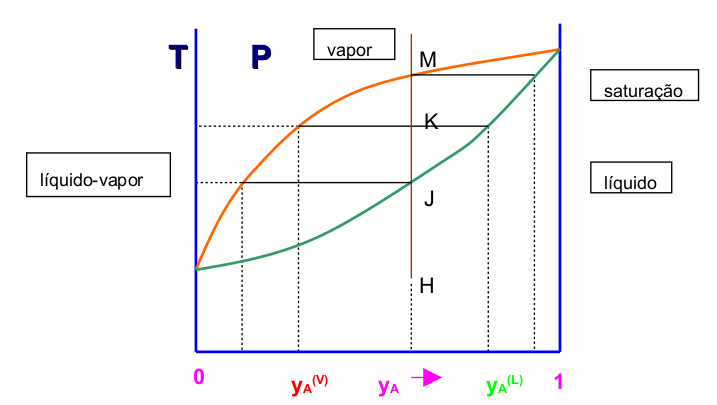
\includegraphics[
            width=0.75\textwidth
        ]   {phaseDiagramBinarySystem.png}

        \label{fig:phaseDiagramBinarySystem}
    \end{figure}

    Quando se aquece um líquido de composição \propcomp{moleFraction}{A} a
    partir do ponto H, ao chegar no ponto J, surge a primeira bolha de vapor
    com uma concentração bastante elevada de B. O lugar geométrico desses
    pontos representa a curva de ponto de bolha.  Desse ponto J em diante vão
    se alterando as concentrações de A (e de B) tanto na fase do líquido como
    na do vapor. Quando passar pelo ponto K, as concentrações no vapor e no
    líquido serão \phase{\propcomp{moleFraction}{A}}{V} e
    \phase{\propcomp{moleFraction}{A}}{L} respectivamente. Chegando ao ponto M,
    desaparecerá a última gota de líquido, que terá uma elevada concentração de
    A. A linha que une esses pontos é denominada curva de ponto de orvalho. Daí
    em diante, se continuarmos aumentando a temperatura do sistema, obteremos
    somente vapor cuja concentração será a mesma concentração original
    \propcomp{moleFraction}{A}, é claro.

    Note que as concentrações de A (e de B) foram definidas dentro de cada fase
    e, portanto, concentrações em fases diferentes não estão diretamente
    relacionadas (não se somam, por exemplo). Perceba, também, que quando
    \propcomp{moleFraction}{A} é igual a zero, trata-se de B puro e, portanto,
    a temperatura desse ponto corresponde simplesmente à temperatura de
    saturação à pressão P. Por raciocínio análogo, quando
    \propcomp{moleFraction}{A} é igual à unidade, trata-se da temperatura de
    saturação de A puro em P. Notemos, de passagem, que B é mais volátil do que
    A (por quê?), um fato importante quando desejamos separar B e A por
    destilação. Pense em etanol e água, por exemplo.

    Aumentando-se a pressão, as curvas que encerram a região de saturação se
    deslocam para cima e seu limite é estabelecido por uma envoltória limitada
    à esquerda e à direita pelos pontos críticos de B e de A (Você sabe dizer
    por quê?).

    Uma seção de temperatura constante enquanto se varia a pressão do sistema,
    revela um cenário similar ao descrito no que se refere às concentrações
    de A (e de B) no líquido e no vapor.

    Existem sistemas binários bifásicos nos quais, sob uma concentração bem
    definida, o líquido passa diretamente para a fase vapor como se fosse uma
    substância pura. Estas são as \emph{misturas azeotrópicas}, que tem tido
    importância crescente como fluidos refrigerantes, para substituir os
    fluoro-carbonados.

    Os diagramas de fase do tipo da \cref{fig:phaseDiagramBinarySystem} são
    adequados para líquidos e vapores miscíveis em todas as proporções. Se os
    líquidos forem parcialmente miscíveis, mas imiscíveis em grandes
    concentrações tanto de A em B, como de B em A, o diagrama exibirá mais duas
    fases, com mostra a \cref{fig:phaseDiagramaPartMiscibleLiquids}.

    \begin{figure}[!htb]
        \caption{%
            Diagrama de fases para líquidos parcialmente miscíveis.
        }

        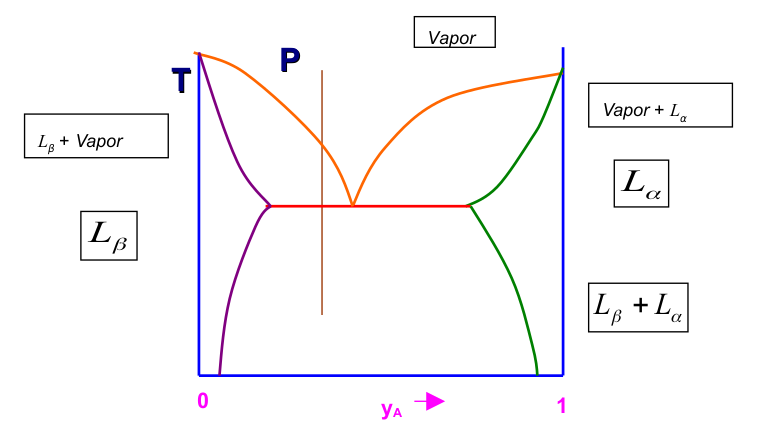
\includegraphics[
            width=0.75\textwidth
        ]   {phaseDiagramaPartMiscibleLiquids.png}

        \label{fig:phaseDiagramaPartMiscibleLiquids}
    \end{figure}

    Observe que no caso dos diagramas do tipo da
    \cref{fig:phaseDiagramaPartMiscibleLiquids}, existirão várias regiões
    bifásicas $L_\beta + L_\alpha$, $L_\beta +$ vapor, vapor $+ L_\alpha$ e um
    ponto trifásico (onde está?), onde as três fases convivem em equilíbrio.

    Uma discussão completamente análoga pode ser apresentada para sistemas
    binários em líquidos, sólidos e na região bifásica líquido + sólido.

    Estes são aspectos qualitativos ou até mesmo obtidos experimentalmente.
    Gostaríamos, entretanto, de sermos capazes de modelar quantitativamente o
    equilíbrio de fases. Para isso, precisaremos da propriedade termodinâmica
    fugacidade, que para o caso de substância pura foi definida na
    \cref{sec:fugacityDefintion}.

    Seja o caso de um único componente em equilíbrio líquido-vapor. Então, da
    \cref{eq:9.15} e da definição de fugacidade de substância pura, obtemos:
    %
    \begin{equation} \label{eq:9.24}
        \propcomp{fugacity}{\gls{satLiquid}}
        \functionOf{
            \gls{temperature},
            \gls{pressure}
        }
        =
        \propcomp{fugacity}{\gls{satVapor}}
        \functionOf{
            \gls{temperature},
            \gls{pressure}
        }
    \end{equation}

    Já sabemos que existe uma relação entre \gls{pressure} e \gls{temperature}.
    Além disso, observe que a \cref{eq:9.24} é razão pela qual não existem
    linhas separadas de liquido saturado e de vapor saturado (um domo de
    vapor), como é o caso da entalpia e da entropia. Se o vapor saturado
    estiver na região de gás perfeito a \gls{temperature}:
    %
    \begin{equation} \label{eq:9.25}
        \propcomp{fugacity}{\gls{satLiquid}}
        =
        \propcomp{fugacity}{\gls{satVapor}}
        =
        \gls{satPressure}
        \functionOf{
            \gls{temperature}
        }\,.
    \end{equation}

    A fugacidade do líquido comprimido
    \gsub{fugacity}{compressedLiquid}\functionOf{\gls{temperature},
    \gls{pressure}} (e do sólido) pode ser obtida integrando-se a
    \cref{eq:6.21} desde \gls{satPressure}\functionOf{\gls{temperature}} a um
    \gls{pressure} qualquer, mantendo-se a temperatura \gls{temperature} constante:
    %
    \begin{equation} \label{eq:9.26}
        \ln{
            \left(
                \frac{
                    \gsub{fugacity}{compressedLiquid}
                    \functionOf{
                        \gls{temperature},
                        \gls{pressure}
                    }
                }{
                    \propcomp{fugacity}{\gls{satLiquid}}
                    \functionOf{
                        \gls{temperature}
                    }
                }
            \right)
        }_{\gls{temperature}}
        =
        \int\limits_{
            \gls{satPressure}
            \functionOf{
                \gls{temperature}
            }
        }^{
            \gls{pressure}
        }{
            \frac{
                \molar{\gls{specificVolume}}
                \functionOf{
                    \gls{temperature},
                    \gls{pressure}
                }
            }{
                \gls{universalGasConstant}
                \gls{temperature}
            }
        }\diff{\gls{pressure}}_{\gls{temperature}}\,.
    \end{equation}

    Vamos definir o Fator de Poynting \gls{PoyntingFactor} como sendo
    %
    \begin{equation} \label{eq:9.27}
        \gls{PoyntingFactor}
        \functionOf{
            \gls{temperature},
            \gls{pressure}
        }
        =
        \mathrm{exp}{
            \left(
            \displaystyle
            \int\limits_{
                \gls{satPressure}
                \functionOf{
                    \gls{temperature}
                }
            }^{
                \gls{pressure}
            }
            \frac{
                \molar{\gls{specificVolume}}
                \functionOf{
                    \gls{temperature},
                    \gls{pressure}
                }
            }{
                \gls{universalGasConstant}
                \gls{temperature}
            }\diff{\gls{pressure}}_{\gls{temperature}}
            \right)
        }\,.
    \end{equation}

    Como \molar{\gls{specificVolume}} de sólidos e líquidos é muito pequeno,
    podemos ainda, se as diferenças de pressão não forem muito grandes,
    aproximar a \cref{eq:9.27} por:
    %
    \begin{equation} \label{eq:9.28}
        \gls{PoyntingFactor}
        \functionOf{
            \gls{temperature},
            \gls{pressure}
        }
        \simeq
        \mathrm{exp}{
            \displaystyle
            \left[
                \frac{
                    \molar{\gls{specificVolume}}
                }{
                    \gls{universalGasConstant}
                    \gls{temperature}
                }
                \left(
                    \gls{pressure}
                    -
                    \gls{satPressure}
                \right)
            \right]
        }
        \simeq 1\,.
    \end{equation}

    Substituindo-se \gls{PoyntingFactor} na \cref{eq:9.26} e rearranjando-se:
    %
    \begin{equation} \label{eq:9.29}
        \gsub{fugacity}{compressedLiquid}
        \functionOf{
            \gls{pressure},
            \gls{temperature}
        }
        =
        \propcomp{fugacity}{\gls{satLiquid}}
        \functionOf{
            \gls{temperature}
        }
        \gls{PoyntingFactor}
        \functionOf{
            \gls{temperature},
            \gls{pressure}
        }
        \simeq
        \propcomp{fugacity}{\gls{satLiquid}}
        \functionOf{
            \gls{temperature}
        }\,,
    \end{equation}
    %
    donde concluímos ainda que, se o vapor saturado for gás perfeito
    %
    \begin{equation} \label{eq:9.30}
        \gsub{fugacity}{compressedLiquid}
        \functionOf{
            \gls{pressure},
            \gls{temperature}
        }
        =
        \propcomp{fugacity}{\gls{satLiquid}}
        \gls{PoyntingFactor}
        =
        \propcomp{fugacity}{\gls{satVapor}}
        \gls{PoyntingFactor}
        =
        \gls{satPressure}
        \functionOf{
            \gls{temperature}
        }
        \gls{PoyntingFactor}
        \simeq
        \gls{satPressure}
        \functionOf{
            \gls{temperature}
        }\,,
    \end{equation}
    %
    e mediante raciocínio análogo, você pode mostrar que o mesmo vale para a
    fugacidade de sólidos e a saturação sólido-vapor de uma substância pura.


    \section{A Fugacidade no Equilíbrio de Fases}

    Consideremos um sistema binário bifásico a
    \gls{temperature},\gls{pressure}.  Então, vimos pelas
    \cref{eq:9.11,eq:9.12} que podemos expressar o equilíbrio das fases 1 e 2
    por:
    %
    \begin{equation*}
        \begin{aligned}
        \phase{\partmolalprop{GibbsFreeEnergy}{A}}{1}
        \functionOf{
            \gls{temperature},
            \gls{pressure},
            \phase{\propcomp{moleFraction}{A}}{1}
        }
        &=
        \phase{\partmolalprop{GibbsFreeEnergy}{A}}{2}
        \functionOf{
            \gls{temperature},
            \gls{pressure},
            \phase{\propcomp{moleFraction}{A}}{2}
        }\,,\\
        %
        \phase{\partmolalprop{GibbsFreeEnergy}{B}}{1}
        \functionOf{
            \gls{temperature},
            \gls{pressure},
            \phase{\propcomp{moleFraction}{A}}{1}
        }
        &=
        \phase{\partmolalprop{GibbsFreeEnergy}{B}}{2}
        \functionOf{
            \gls{temperature},
            \gls{pressure},
            \phase{\propcomp{moleFraction}{A}}{2}
        }\,,
        \end{aligned}
    \end{equation*}
    %
    ou
    %
    \begin{equation*}
        \begin{aligned}
        \phase{\propcomp{chemicalPotential}{A}}{1}
        \functionOf{
            \gls{temperature},
            \gls{pressure},
            \phase{\propcomp{moleFraction}{A}}{1}
        }
        &=
        \phase{\propcomp{chemicalPotential}{A}}{2}
        \functionOf{
            \gls{temperature},
            \gls{pressure},
            \phase{\propcomp{moleFraction}{A}}{2}
        }\,,\\
        %
        \phase{\propcomp{chemicalPotential}{B}}{1}
        \functionOf{
            \gls{temperature},
            \gls{pressure},
            \phase{\propcomp{moleFraction}{A}}{1}
        }
        &=
        \phase{\propcomp{chemicalPotential}{B}}{2}
        \functionOf{
            \gls{temperature},
            \gls{pressure},
            \phase{\propcomp{moleFraction}{A}}{2}
        }\,,
        \end{aligned}
    \end{equation*}
    %
    de onde concluímos que
    %
    \begin{equation} \label{eq:9.33}
        \begin{aligned}
        \left(
            \diff\phase{\partmolalprop{GibbsFreeEnergy}{A}}{1}
        \right)_{\gls{temperature}}
        &=
        \left(
            \phase{\partmolalprop{GibbsFreeEnergy}{A}}{2}
        \right)_{\gls{temperature}}\,,\\
        %
        \left(
            \diff\phase{\partmolalprop{GibbsFreeEnergy}{B}}{1}
        \right)_{\gls{temperature}}
        &=
        \left(
            \phase{\partmolalprop{GibbsFreeEnergy}{B}}{2}
        \right)_{\gls{temperature}}\,,\\
        \end{aligned}
    \end{equation}
    %
    e, substituindo-se pelas fugacidades na mistura a \gls{temperature} e
    \gls{pressure},
    %
    \begin{equation} \label{eq:9.34}
        \begin{aligned}
        \phase{\partmolalprop{fugacity}{A}}{1}
        \functionOf{
            \gls{temperature},
            \gls{pressure},
            \phase{\propcomp{moleFraction}{A}}{1}
        }
        &=
        \phase{\partmolalprop{fugacity}{A}}{2}
        \functionOf{
            \gls{temperature},
            \gls{pressure},
            \phase{\propcomp{moleFraction}{A}}{2}
        }\,,\\
        %
        \phase{\partmolalprop{fugacity}{B}}{1}
        \functionOf{
            \gls{temperature},
            \gls{pressure},
            \phase{\propcomp{moleFraction}{A}}{1}
        }
        &=
        \phase{\partmolalprop{fugacity}{B}}{2}
        \functionOf{
            \gls{temperature},
            \gls{pressure},
            \phase{\propcomp{moleFraction}{A}}{2}
        }\,,
        \end{aligned}
    \end{equation}
    %
    ou seja, o equilíbrio químico é obtido quando, para todos os componentes
    que participam do equilíbrio, a fugacidade de cada componente em cada fase
    é igual à fugacidade do mesmo componente em cada uma das fases.

    De modo geral, para uma mistura de n componentes e p fases:
    %
    \begin{equation} \label{eq:9.35}
        \begin{aligned}
            &\phase{\molalpropcomp{fugacity}{1}}{1}
            \functionOf{
                \gls{temperature},
                \gls{pressure},
                \phase{\propcomp{moleFraction}{1}}{1},
                \hdots,
                \phase{
                    \propcomp{moleFraction}{\gls{numberSpecies} - 1}
                }{1}
            }
            =
            \phase{\molalpropcomp{fugacity}{1}}{2}
            \functionOf{
                \gls{temperature},
                \gls{pressure},
                \phase{\propcomp{moleFraction}{1}}{2},
                \hdots,
                \phase{
                    \propcomp{moleFraction}{\gls{numberSpecies} - 1}
                }{2}
            }
            =
            \hdots
            =
            \phase{\molalpropcomp{fugacity}{1}}{\gls{numberPhases}}
            \functionOf{
                \gls{temperature},
                \gls{pressure},
                \phase{\propcomp{moleFraction}{1}}{\gls{numberPhases}},
                \hdots,
                \phase{
                    \propcomp{moleFraction}{\gls{numberSpecies} - 1}
                }{\gls{numberPhases}}
            }\,,\\
            &\phase{\molalpropcomp{fugacity}{2}}{1}
            \functionOf{
                \gls{temperature},
                \gls{pressure},
                \phase{\propcomp{moleFraction}{1}}{1},
                \hdots,
                \phase{
                    \propcomp{moleFraction}{\gls{numberSpecies} - 1}
                }{1}
            }
            =
            \phase{\molalpropcomp{fugacity}{2}}{2}
            \functionOf{
                \gls{temperature},
                \gls{pressure},
                \phase{\propcomp{moleFraction}{1}}{2},
                \hdots,
                \phase{
                    \propcomp{moleFraction}{\gls{numberSpecies} - 1}
                }{2}
            }
            =
            \hdots
            =
            \phase{\molalpropcomp{fugacity}{2}}{\gls{numberPhases}}
            \functionOf{
                \gls{temperature},
                \gls{pressure},
                \phase{\propcomp{moleFraction}{1}}{\gls{numberPhases}},
                \hdots,
                \phase{
                    \propcomp{moleFraction}{\gls{numberSpecies} - 1}
                }{\gls{numberPhases}}
            }\,,\\
            &\vdots\\
            &\phase{\molalpropcomp{fugacity}{\gls{numberSpecies}}}{1}
            \functionOf{
                \gls{temperature},
                \gls{pressure},
                \phase{\propcomp{moleFraction}{1}}{1},
                \hdots,
                \phase{
                    \propcomp{moleFraction}{\gls{numberSpecies} - 1}
                }{1}
            }
            =
            \phase{\molalpropcomp{fugacity}{\gls{numberSpecies}}}{2}
            \functionOf{
                \gls{temperature},
                \gls{pressure},
                \phase{\propcomp{moleFraction}{1}}{2},
                \hdots,
                \phase{
                    \propcomp{moleFraction}{\gls{numberSpecies} - 1}
                }{2}
            }
            =
            \hdots
            =
            \phase{
                \molalpropcomp{fugacity}{\gls{numberSpecies}}
            }{\gls{numberPhases}}
            \functionOf{
                \gls{temperature},
                \gls{pressure},
                \phase{\propcomp{moleFraction}{1}}{\gls{numberPhases}},
                \hdots,
                \phase{
                    \propcomp{moleFraction}{\gls{numberSpecies} - 1}
                }{\gls{numberPhases}}
            }\,,\\
        \end{aligned}
    \end{equation}
    %
    com as variáveis
    %
    \begin{equation}
        \gls{temperature},
        \gls{pressure},
        \phase{\propcomp{moleFraction}{1}}{1},
        \phase{\propcomp{moleFraction}{2}}{1},
        \hdots,
        \phase{\propcomp{moleFraction}{\gls{numberSpecies} - 1}}{1},
        \phase{\propcomp{moleFraction}{1}}{2},
        \phase{\propcomp{moleFraction}{2}}{2},
        \hdots,
        \phase{\propcomp{moleFraction}{\gls{numberSpecies} - 1}}{2},
        \hdots,
        \phase{\propcomp{moleFraction}{1}}{\gls{numberPhases}},
        \phase{\propcomp{moleFraction}{2}}{\gls{numberPhases}},
        \hdots,
        \phase{
            \propcomp{moleFraction}{\gls{numberSpecies} - 1}
        }{\gls{numberPhases}}\,.
    \end{equation}

    % Comment: eq. 9.39ainda não definida neste ponto do texto
    Bem, embora a formulação da \cref{eq:9.39} seja bastante geral, ainda não
    podemos determinar quantitativamente o equilíbrio sem um modelo para as
    fugacidades de cada componente na mistura homogênea de cada fase.
    Aproveitando o nosso conhecimento sobre misturas homogêneas, vamos estudar
    alguns modelos a partir da solução ideal, da mistura de gases perfeitos e
    finalmente da mistura como pseudo-substância pura.


    \section{O Modelo de Solução Ideal para o Equilíbrio}

    Pode-se demonstrar que, para uma mistura homogênea que se comporta como
    solução ideal a \gls{temperature},\gls{pressure}:
    %
    \begin{equation} \label{eq:9.36}
        \molalpropcomp{fugacity}{i}
        =
        \propcomp{moleFraction}{i}
        \propcomp{fugacity}{i}
        \functionOf{
            \gls{temperature},
            \gls{pressure}
        }\,,
    \end{equation}
    %
    para todos os componentes $i$ da solução ideal. Já conhecemos esta relação
    entre a fugacidade do componente na mistura e a fugacidade do componente
    puro. Esta é conhecida como a \emph{Relação de Lewis-Randall}.

    Consideremos um sistema binário bifásico de A e B, em equilíbrio
    líquido-vapor a \gls{temperature},\gls{pressure}. Vamos admitir que tanto o
    líquido como o vapor se comportam como soluções ideais. Então, substituindo
    a relação de Lewis-Randall nas equações de equilíbrio, temos

    \begin{equation} \label{eq:9.37}
        \begin{aligned}
            \phase{\propcomp{moleFraction}{A}}{L}
            \phase{\propcomp{fugacity}{A}}{L}
            \functionOf{
                \gls{temperature},
                \gls{pressure}
            }
            &=
            \phase{\propcomp{moleFraction}{A}}{V}
            \phase{\propcomp{fugacity}{A}}{V}
            \functionOf{
                \gls{temperature},
                \gls{pressure}
            }\\
            \left(
                1 - \phase{\propcomp{moleFraction}{A}}{L}
            \right)
            \phase{\propcomp{fugacity}{B}}{L}
            \functionOf{
                \gls{temperature},
                \gls{pressure}
            }
            &=
            \left(
                1 - \phase{\propcomp{moleFraction}{A}}{V}
            \right)
            \phase{\propcomp{fugacity}{B}}{V}
            \functionOf{
                \gls{temperature},
                \gls{pressure}
            }\,.
        \end{aligned}
    \end{equation}

    As variáveis são
    $\gls{temperature}, \gls{pressure}, \phase{\propcomp{moleFraction}{A}}{L},
    \phase{\propcomp{moleFraction}{A}}{V}$.  Observe que, se conhecermos
    $\gls{temperature},\gls{pressure}$ podemos, em princípio, determinar as
    fugacidades das substâncias puras A e B. O problema é que nós temos duas
    fugacidades distintas, uma para cada fase L e V, para o mesmo
    \gls{temperature},\gls{pressure}. Temos, então, que lançar mão de estados
    hipotéticos! Vamos discutir um exemplo: água pura a \SI{25}{\celsius} e
    \SI{0.1}{\mega\pascal} está, como já vimos anteriormente, em um estado de
    líquido (levemente) comprimido, ao passo que água naquelas mesmas
    condições, mas em forma de gás, só pode ser um estado hipotético...

    Se você não entendeu o aparecimento do estado hipotético da água, considere
    o ar úmido, que é ar seco misturado com vapor de água. Se este ar úmido
    estiver em equilíbrio com a água (A) líquida a $\gls{temperature} =
    \SI{25}{\celsius}$ e $\gls{pressure} = \SI{0.1}{\mega\pascal}$, então,
    aplicando-se a Lei de Lewis-Randall somente para a água (por que não
    aplicamos para o ar seco também?):
    %
    \begin{equation} \label{eq:9.38}
        \phase{\propcomp{moleFraction}{A}}{V}
        \phase{\propcomp{fugacity}{A}}{V}
        \functionOf{
            \gls{temperature},
            \gls{pressure}
        }
        =
        \phase{\propcomp{fugacity}{A}}{L}
        \functionOf{
            \gls{temperature},
            \gls{pressure}
        }\,.
    \end{equation}

    Sabemos que a fugacidade da água como líquido comprimido a
    \gls{temperature},\gls{pressure} , onde F é o Fator de Poynting, pode ser
    expressa por:
    %
    \begin{equation} \label{eq:9.39}
        \phase{\propcomp{fugacity}{A}}{L}
        \functionOf{
            \gls{temperature},
            \gls{pressure}
        }
        =
        \gls{satPressure}
        \functionOf{
            \gls{temperature}
        }
        \gls{PoyntingFactor}
        \simeq
        \gls{satPressure}
        \functionOf{
            \gls{temperature}
        }\,.
    \end{equation}

    Veja bem: a fugacidade da água líquida pura a
    \gls{temperature},\gls{pressure}, que é líquido levemente comprimido, é
    aproximadamente igual à pressão de saturação em \gls{temperature}. Por outro, lado, qual
    seria a fugacidade da água pura como vapor (V) a
    \gls{temperature},\gls{pressure}? Estamos claramente diante de um estado
    hipotético da água... A fugacidade da água na fase vapor, se puder ser
    considerada como gás perfeito a \gls{temperature},\gls{pressure} ficará:
    %
    \begin{equation} \label{eq:9.40}
        \phase{\propcomp{fugacity}{A}}{V}
        \functionOf{
            \gls{temperature},
            \gls{pressure}
        }
        =
        \gls{pressure}
    \end{equation}
    %
    de forma que a equação do equilíbrio \cref{eq:9.39} se torna:
    %
    \begin{equation} \label{eq:9.41}
        \phase{\propcomp{moleFraction}{A}}{V}
        \gls{pressure}
        =
        \propcomp{satPressure}{A}
        \functionOf{
            \gls{temperature}
        }
        \gls{PoyntingFactor}
        \simeq
        \propcomp{satPressure}{A}
        \functionOf{
            \gls{temperature}
        }\,,
    \end{equation}
    %
    ou seja, a pressão parcial que a água exerce no ar úmido considerado como
    uma mistura de gases perfeitos em equilíbrio a
    \gls{temperature},\gls{pressure} com a água líquida é praticamente igual a
    pressão de saturação da água pura na temperatura \gls{temperature}. Você
    consegue entender agora a diferença entre a saturação líquido-vapor de uma
    substância pura e a saturação daquela mesma substância com o líquido na
    presença de seu vapor acrescido de um gás não condensável?


    \section{O Modelo Regra de Raoult-Gás Perfeito}

    O desenvolvimento anterior nos dá a pista para evitarmos os estados
    hipotéticos no equilíbrio líquido-vapor: Basta considerarmos a fase vapor
    como se fosse gás perfeito. Assim, juntando o modelo de solução ideal com
    gás perfeito, obtemos, para um sistema binário bifásico a
    \gls{temperature},\gls{pressure} em equilíbrio líquido-vapor:
    %
    \begin{equation} \label{eq:9.42}
        \begin{aligned}
        \phase{\propcomp{moleFraction}{A}}{L}
        \propcomp{satPressure}{A}
        \functionOf{
            \gls{temperature}
        }
        &=
        \phase{\propcomp{moleFraction}{A}}{V}
        \gls{pressure}\\
        \left(
            1 - \phase{\propcomp{moleFraction}{A}}{L}
        \right)
        \propcomp{satPressure}{B}
        \functionOf{
            \gls{temperature}
        }
        &=
        \left(
            1 - \phase{\propcomp{moleFraction}{A}}{V}
        \right)
        \gls{pressure}\,,
        \end{aligned}
    \end{equation}
    %
    que representa um sistema de duas equações a quatro incógnitas. Se
    fornecermos \gls{temperature},\gls{pressure}, então seremos capazes de
    determinar todas as concentrações de A e B, tanto  na fase líquida, como na
    fase vapor. Este é o modelo da Regra de Raoult-gás perfeito, que é simples
    e funciona razoavelmente bem apenas para pressões moderadas. Reveja o
    exemplo anterior do ar úmido saturado e você se dará conta de que
    utilizamos a Regra de Raoult-gás perfeito para resolvê-lo.

    \section{Psicrometria}

    Veja o texto, programa de computador e exemplos nas figuras incluídas
    adiante.
